% mnras_template.tex
%
% LaTeX template for creating an MNRAS paper
%
% v3.0 released 14 May 2015
% (version numbers match those of mnras.cls)
%
% Copyright (C) Royal Astronomical Society 2015
% Authors:
% Keith T. Smith (Royal Astronomical Society)

% Change log
%
% v3.0 May 2015
%    Renamed to match the new package name
%    Version number matches mnras.cls
%    A few minor tweaks to wording
% v1.0 September 2013
%    Beta testing only - never publicly released
%    First version: a simple (ish) template for creating an MNRAS paper

%%%%%%%%%%%%%%%%%%%%%%%%%%%%%%%%%%%%%%%%%%%%%%%%%%
% Basic setup. Most papers should leave these options alone.
\documentclass[a4paper,fleqn,usenatbib]{mnras}

% MNRAS is set in Times font. If you don't have this installed (most LaTeX
% installations will be fine) or prefer the old Computer Modern fonts, comment
% out the following line
\usepackage{newtxtext,newtxmath}
% Depending on your LaTeX fonts installation, you might get better results with one of these:
%\usepackage{mathptmx}
%\usepackage{txfonts}

% Use vector fonts, so it zooms properly in on-screen viewing software
% Don't change these lines unless you know what you are doing
\usepackage[T1]{fontenc}
\usepackage{ae,aecompl}


%%%%% AUTHORS - PLACE YOUR OWN PACKAGES HERE %%%%%

% Only include extra packages if you really need them. Common packages are:
\usepackage{graphicx}	% Including figure files
\usepackage{amsmath}	% Advanced maths commands
\usepackage{amssymb}	% Extra maths symbols
\usepackage{deluxetable}


%%%%%%%%%%%%%%%%%%%%%%%%%%%%%%%%%%%%%%%%%%%%%%%%%%

%%%%% AUTHORS - PLACE YOUR OWN COMMANDS HERE %%%%%

% Please keep new commands to a minimum, and use \newcommand not \def to avoid
% overwriting existing commands. Example:
%\newcommand{\pcm}{\,cm$^{-2}$}	% per cm-squared

%%%%%%%%%%%%%%%%%%%%%%%%%%%%%%%%%%%%%%%%%%%%%%%%%%

%%%%%%%%%%%%%%%%%%% TITLE PAGE %%%%%%%%%%%%%%%%%%%

% Title of the paper, and the short title which is used in the headers.
% Keep the title short and informative.
\title[Mid--IR RR Lyrae PL Relation in $\omega$ Cen]{The Carnegie RR Lyrae Program: The Mid--Infrared RR Lyrae Period-Luminosity Relation in $\omega$ Centuri}

% The list of authors, and the short list which is used in the headers.
% If you need two or more lines of authors, add an extra line using \newauthor
\author[V. Scowcroft et al.]{
Victoria Scowcroft$^{1}$\thanks{E-mail: vs@obs.carnegiescience.edu}
Meredith Durbin$^{2, 3}$
Wendy Freedman$^{4}$
Gurtina Besla$^{5}$ 
\newauthor Giuseppe Bono$^{6, 7}$
Maria--Rosa Cioni$^{8, 9, 10}$
Gisella Glementini$^{11}$
Kathryn Johnston$^{12}$
\newauthor Nitya Kallivayalil$^{13}$
Juna Kollmeier$^{1}$
David Law$^{3}$
Barry Madore$^{1}$
Steve Majewski$^{13}$
\newauthor Roeland van der Marel$^{3}$
Massimo Marengo$^{14}$
Andrew~J.~Monson$^{1}$
David Nidever$^{15}$ 
\newauthor S.~E.~Persson$^{1}$
Grzegorz Pietrzynski$^{16, 17}$
George Preston$^{1}$
Mark Seibert$^{1}$
Horace Smith$^{18}$
\newauthor Igor Soszynski$^{16}$
Ian Thompson$^{1}$
Andrzej Udalski$^{16}$
\\
% List of institutions
$^1$Observatories of the Carnegie Institution of Washington, 813 Santa Barbara St., Pasadena, CA 91101, USA \\
$^2$Pomona College, Claremont, CA 91711, USA \\
$^3$ Space Telescope Science Institute, 3700 San Martin Drive, Baltimore, MD 21218, USA \\
$^4$ Department of Astronomy and Astrophysics, University of Chicago, 5640 S Ellis Ave, Chicago, IL 60637, USA \\
$^5$ Department of Astronomy and Steward Observatory, University of Arizona, 933 North Cherry Avenue,   Tucson, AZ 85721, USA \\
$^6$ Univ. Roma ``Tor Vergata", Via della Ricerca Scientifica, 1 � 00133, Roma, Italy \\
$^7$ INAF�OAR, via Frascati 33 � 00040, Monte Porzio Catone (RM), Italy \\
$^8$ Universtat Potsdam, Institut fur Physik und Astronomie, Karl-Liebknecht-Str. 24/25, 14476 Potsdam, Germany \\
$^9$ Leibniz-Institut fur Astrophysik Potsdam, An der Sternwarte 16, 14482 Potsdam, Germany \\
$^{10}$ University of Hertfordshire, Physics, Astronomy and Mathematics, College Lane, Hatfield AL10 9AB, United Kingdom \\
$^{11}$ INAF - Osservatorio Astronomico, Via Ranzani n. 1, 40127 Bologna, Italy \\
$^{12}$ Department of Astronomy, Columbia University, New York, NY 10027, USA  \\
$^{13}$ Department of Astronomy, University of Virginia, Charlottesville, VA 22904-0818, USA \\
$^{14}$ Department of Physics and Astronomy, Iowa State University, Ames, IA, USA \\
$^{15}$ Department of Astronomy, University of Michigan, Ann Arbor, MI 48109, USA \\
$^{16}$ Warsaw University Observatory Al. Ujazdowskie 4, 00-478 Warszawa, Poland \\
$^{17}$ Departamento de Astronomia, Universidad de Concepcion, Casilla 160-C, Chile \\
$^{18}$ Department of Physics and Astronomy, Michigan State University, East Lansing, MI, USA 48824 \\
}

% These dates will be filled out by the publisher
\date{Accepted XXX. Received YYY; in original form ZZZ}

% Enter the current year, for the copyright statements etc.
\pubyear{2015}

% Don't change these lines
\begin{document}
\label{firstpage}
\pagerange{\pageref{firstpage}--\pageref{lastpage}}
\maketitle

% Abstract of the paper
\begin{abstract}
We present new period-luminosity relations for RR Lyrae variables in 3.6 and 4.5 \micron\ derived from time-resolved IRAC data of $\omega$ Centauri. The sample consists of 36 RR Lyrae in 3.6 \micron\ and 37 in 4.5 \micron, 22 of which appear in both channels and have literature values for metallicities. We find no compelling evidence for a metallicity correlation in the residuals, based on a spread of 1.2 dex in [Fe/H].\end{abstract}

% Select between one and six entries from the list of approved keywords.
% Don't make up new ones.
\begin{keywords}
keyword1 -- keyword2 -- keyword3
\end{keywords}

%%%%%%%%%%%%%%%%%%%%%%%%%%%%%%%%%%%%%%%%%%%%%%%%%%

%%%%%%%%%%%%%%%%% BODY OF PAPER %%%%%%%%%%%%%%%%%%

\section{Introduction}
The Carnegie Hubble Program (CHP) is a Warm \textit{Spitzer} program with the aim of measuring $H_{0}$ to a systematic uncertainty of 3\%, eventually reducing that uncertainty to 2\% using \textit{JWST}. The first part of the CHP used Cepheids as the primary distance indicator, using parallax measurements of Cepheids from \textit{HST} \citep{2007AJ....133.1810B} to calibrate the zero--point of the Cepheid Period--Luminosity (PL) relation (also known as the Leavit Law, or LL), leading out to Cepheid measurements in the Milky Way \citep[MW,][]{2012ApJ...759..146M} and Large Magallanic Cloud \citep[LMC,][]{2011ApJ...743...76S}. An initial recalibration of $H_{0}$ from CHP was presented in \citet{2012ApJ...758...24F}.

The CHP removed many systematics from the $H_{0}$ measurement by moving to the mid--infrared (extinction is reduced by a factor of 16 to 20, amplitude of Cepheid pulsation is reduced, intrinsic width of LL is reduced) and by using a single instrument (no effects from ground--to--space transformation, for example) but there are some effects that cannot be accounted for without further tests. By only using a single distance indicator (i.e. Cepheids) for the zero--point measurement, we have no understanding of the intrinsic accuracy of our measurement. With recent measurements from cosmic microwave background (CMB) experiements such as Planck \citep{	
2015arXiv150201589P} in tension with local $H_{0}$ values, we must assess all possible sources of systematic uncertainty in our measurement. This is where the Carnegie RR Lyrae Program comes into play.

** VS NOTE: With regard to CMB -- is measurements the correct word here? Obviously Planck et al. make measurements, but they do not measure $H_{0}$, it is inferred from a model. What word would be more appropriate here? **

The Carnegie RR Lyrae Program (CRRP) assess a systematic that was unreachable in the original CHP --- the intrinsic accuracy of the mid--infrared Cepheid standard candle distance scale when compared to the standard ruler distance scale of CMB and Baryon Acoustic Oscillation (BAO) measurements. With only one ``test candle'' it is impossible to make any assessment of this accuracy. However, when we have two standard candles with similar precision we can make meaningful comparisons and assess the systematic accuarcy of both of them.

%The Carnegie-Hubble Program is an effort led by the Observatories of the Carnegie Institution of Washington to reduce the total systematic and statistical error in $H_0$ to $\pm 2\%$ or better, and the Carnegie RR Lyrae Program is a branch of the CHP focusing on distance calibration with RR Lyrae. The RR Lyrae distance scale does not extend as far as the Cepheid distance scale, but it is more precise than and rigorously independent of the Cepheid scale, which makes it an excellent candidate for constraining systematic errors in Cepheid distances as well as a valuable calibrator in its own right.

In the past RR Lyrae variables have often been thought of as the poor substitute for Cepheids in terms of distance scale measurements. They are intrinsically fainter, and in the optical follow a much shallower, even horizontal, PL relation. Determining an accurate distance to an RR Lyrae (RRL) in the $V$ band requires knowledge of its [Fe/H] --- a quantity which itself is not  easy to obtain. However, in more recent years near-- and mid--infrared observations have shown the true power of RRL as precision distance indicators. In a similar vein to Cepheids, \text{HST} parallaxes were obtained for serveral Galactic RRL calibrators \citet{2011AJ....142..187B} and several groups have been studying the populations of RRL in globular clusters and nearby dwarf spheriodal galaxies (NEED REFS). 

In the mid--infrared RRL exhibit similar properties to Cepheids\citep{2013ApJ...776..135M}. Their light curve amplitudes are minimised as we are seeing deeper into the star. At the wavelengths observed by Warm \textit{Spitzer} (3.6 and 4.5~$\mu$m) we do not see photospheric effects, but only the effects of temperature driving the pulsation. Essentially, the mid--infrared light curve is tracing the radius change of the star. A by--product of this effect is that the intrinsic width of the RRL PL relation is also minimised in the mid--infrared (mid--IR). The PL relation for pulsational variables can be thought of as a two--dimensional projection of the three--dimensional period--luminosity--colour relation (see figure 3 of \citet{1991PASP..103..933M} for a graphical representation). As the colour--width decreases in the mid--IR, the width of the PL naturally decreases. As one moves from the optical to the mid-IR, the slope of the PL relation steepens and its dispersion dramatically decreases; this phenomenon has been demonstrated in simulations by \citet{2004ApJS..154..633C}, and by several observational efforts, as illustrated in fig. 4 of \citet{2013ApJ...776..135M}. The slope should asymptotically approach the predicted slope of the period-radius relation, resulting in a slope between $-2.4$ and $-2.8$. Through this decrease in dispersion we have found that the intrinsic width of the mid--IR PL for RRL is in fact smaller than for Cepheids --- 0.05~mag compared to 0.10~mag (Monson et al. 2015, Neely et al. 2015). This translates to an uncertainty on an individual RR Lyrae star of 2\%, compared to 4\% for Cepheids. 

In this work we present the mid--IR PL relation for the RRL in the $\omega$~Cen Galactic Globular Cluster (GGC). 
Here we present a mid-infrared of the RR Lyrae period-luminosity (PL) relation in the IRAC channels 1 and 2 centered on 3.6 and 4.5 \micron\ respectively, as well as a preliminary investigation into metallicity effects on the PL relation.

There are very few metallic or molecular transition lines in the mid-IR at typical RR Lyrae temperatures, so the effects of metallicity on luminosity should be minimized. However, $\omega$~Cen provides the ideal test bed for any effect that we may not have predicted. Such an effect is not out of the realm of possibility; for example, the CO band head at 4.5~$\mu$m has been found to have a significant dependence on metallicity, and has such prevented the IRAC 4.5~$\mu$m Cepheid observations from being used for distance measurements in the CHP. As our concern in this program is systematic precision, we must ensure that similar effects do not plague the RRL distance scale.  

$\omega$ Cen in particular is ideal for calibrating the RR Lyrae period-luminosity-metallicity relation, as it contains 192 known RR Lyrae \citep{2004A&A...424.1101K} with a metallicity range spanning over 1.5 dex (Bono 2013, private communication); a metallicity spread this wide is not found in any other GGC. As noted in \citet{2006MNRAS.372.1675S}, one of the advantages of using globular clusters to calibrate PL coefficients is that all stars in a cluster can be considered to be at the same distance from Earth. We can therefore assume that any dispersion in the PL relation is a combination of the a) the intrinsic dispersion of the PL relation, b) the photometric uncertainties, and c) dispersion induced by the spread in metallicity of the RRL. We have measured the intrinsic dispersion of the RRL PL from other clusters (e.g. M4, Neely et al. 2015), and our photometric uncertainties are a well defined \textbf{constraint, value?? what is the correct word?}, so the only unknown in this problem is the dispersion due to the spread in metallicity of the cluster. We are lucky with $\omega$~Cen that we can also take a second approach to establishing the metallicity effect on the RRL PL relation. As it is such a unique object, $\omega$~Cen is extremely well studied and many of its RRL have spectroscopic or photometric metallicities available. As another test of the effect of metallicity, we use these measeurements to assess the $\gamma$ parameter for the GGC, where 
\begin{equation} \label{eqn:gamma}
\gamma = \dfrac {\Delta \text{mag}} {[Fe/H]}\text{,}
\end{equation}

similar to $\gamma$ used to quantify the effect of metallicity on the zero--point of the Cepheid PL relation. 
%% Note to Meredith -- I've changed the text here to correct an incorrect assumption. You originally had the following:
%"one of the advantages of using globular clusters to calibrate PL coefficients is that all stars in a cluster can be considered to be at the same distance from Earth and subject to the same line-of-sight extinction effect across the cluster, and thus we can be confident that the period-luminosity relations we see are intrinsic to the stars."
% We can assume that the stars are all at the same distance for this exercise (although as we get better at measuring distances we'll be able to measure the 3D structure of the clusters using the spread in the PL, like we did in the SMC), BUT we can't assume the line-of-sight extinction is the same over the whole cluster IN EVERY CASE. M4 is a good example of this -- it has a significant extinction gradient across it. What we can do is calculate individual reddenings to every star we're considering by using multiwavelength information.
% I didn't want to just delete this part of the text without explaining why it had gone. 


The paper is set out as follows: Section~\ref{sec:observations} details the observations and data reduction. Section~\ref{sec:pl_relation} describes the mid--IR PL relations and Section~\ref{sec:distance_moduli} discusses the application of these to a distance measurement of  $\omega$~Cen. Section~\ref{sec:metallicity} and Section~\ref{sec:discussion} examine the effect of metallicty on mid--IR observations of RR Lyrae variables and its implications for distance measurements and the extragalactic distance scale. In Section~\ref{sec:conclusions} we present our conclusions.


\section{Observations \& Data Reduction}
\label{sec:observations}
The observations for this work were taken as part of the Warm~\textit{Spitzer} mission as part of the Carnegie RR Lyrae Program (PI W. Freedman, PID 90002). Three fields in $\omega$~Cen were chosen, their positions and the positions of known RR Lyrae are shown in Figure~\ref{fig:omegaCen_fields}. To obtain optimal RRL light curves we chose to observe each field twelve times over approximately 16 hours, roughly corresponding to the period of the longest period RRL we expected to observe in the field. The observations of all three fields were taken on 2013-05-10 and 2013-05-11. Each field was observed using IRAC \citep{2004ApJS..154...10F} with a 30s frame time with a medium scale, gaussian 5--point dither pattern to mitigate any image artifacts. Images were collected in both the 3.6 and 4.5~$\mu$m channels. 

\begin{figure}
\begin{center}
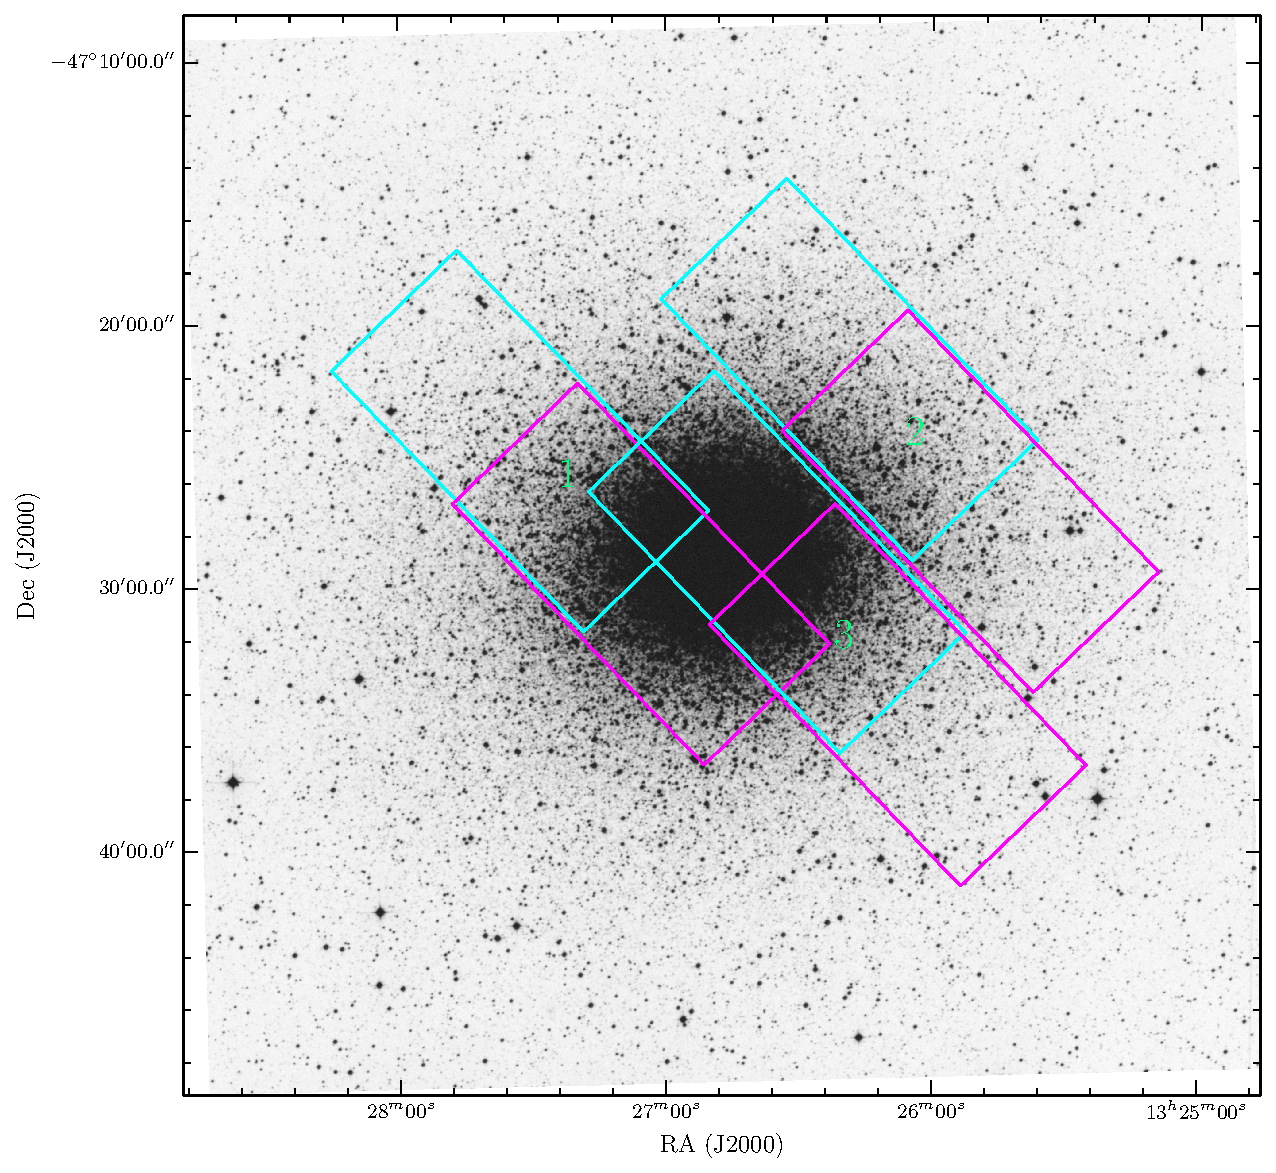
\includegraphics[width=80mm]{omegaCen_figure.pdf}
\caption{DSS2 infra--red image of $\omega$~Cen with the three {\it Spitzer} fields overplotted. The cyan and magenta lines indicate the 3.6~$\mu$m and 4.5~$\mu$m observations respectively. The fields have approximately $1/3$ coverage with at both wavelengths due to the design of the IRAC camera.}
\label{fig:omegaCen_fields}
\end{center}
\end{figure}


The science images were created using \textsc{mopex} \citep{2006SPIE.6274E..0CM}, first running overlap correction on the corrected BCDs (cBCDs) then mosaicking them at 0.6 arcsec pixel scale using the drizle algorithm. Mosaicked location--correction images were created at the same time. 



PSF photometry was performed in PyRAF 2.0 using the \textsc{daophot} package. Initial aperture photometry was performed with an aperture radius of 3.6\arcsec and annulus radius of 4.8\arcsec, whereas the standard IRAC aperture is 6\arcsec; a correction factor of 1.12841 and 1.12738 for 3.6 and 4.5 \micron\ respectively was applied to the instrumental magnitudes. We also calibrate the magnitudes from images in counts (required for \textsc{daophot}) back to flux magnitudes by performing aperture photometry on a set of bright, isolated stars in the flux images, finding the mean difference between the aperture flux magnitudes and PSF counts magnitudes of the same stars, and subtracting said difference from all PSF magnitudes. We also correct for location in the frame using the mosaicked correction images created by \textsc{mopex}




The primary limiting factor in this data is crowding: 77 RR Lyrae out of 192 were rejected due to crowding. To decide which stars to reject, a $K$-band image from the Magellan telescope at Las Campanas Observatory was used, as it provided a full view of the entire cluster, and the most crowded regions were more obvious than in the Spitzer data, although the bandpasses are close enough that they are still comparable. The selection of which stars to reject was made on a primarily visual basis.


\section{Period-Luminosity Relations}
\label{sec:pl_relations}

It is common practice to convert the RRc periods to fundamental mode periods (to ``fundamentalize" them) using the ratio observed in double mode RR Lyrae, where $P_1/P_0 = 0.74432 \pm 0.00003$ or $\log P_0 = \log P_1 + 0.128$ \citep{1996AJ....112.2026W}, such that the types can be combined for a larger sample size, as done in \citet{2004ApJ...610..269D}. \citet{2014MNRAS.440L..96K} present separate relations for each type, arguing that the combination of the types is physically inappropriate, whereas \citet{2014MNRAS.439.3765D} argue that RRc stars exhibit a $K$-band period-luminosity relation that differs from RRab's only by the period shift, and that this should not change in longer wavelengths. Here we have chosen to fundamentalize the RRc periods to maximize our sample sizes; we see no obvious evidence that the types should be separated.

We present PL relations of the form \begin{equation}m = \alpha_\lambda(\pm \sigma_{\alpha_\lambda}) \times \log P + \beta_\lambda(\pm \sigma_{\beta_\lambda})\end{equation}
where $m_\lambda$ is the apparent magnitude in wavelength $\lambda$, $\alpha_\lambda$ is the slope in the same wavelength, $\sigma_{\alpha_\lambda}$ is the error in the slope, $\beta_\lambda$ is the apparent zero point, and $\sigma_{\beta_\lambda}$ is the error in the zero point; we also include formal scatter $\sigma_\lambda$, the standard deviation of the residuals $m_{\text{observed}} - m_{\text{predicted}}$. Here we have weighted the linear fits by individual magnitude errors. See Table~\ref{tab:plparams} for the PL parameters we have derived.

These slopes agree within uncertainty with the slopes of the $W1$ (3.4 \micron) and $W2$ (4.6 \micron) absolute PL relations derived by \citet{2013ApJ...776..135M}, \citet{2014MNRAS.440L..96K}, and \citet{2014MNRAS.439.3765D}; our [4.5] slope in particular is in excellent agreement with Klein et al. (It should be noted that Klein et al. present separate PL relations for RRab's and RRc's; here we are comparing to their RRab slope.) Our formal scatter measurements agree with those of Madore et al. 

The scatter in these PL relations is higher than we expect the intrinsic scatter in these bands to be. Some factors that may contribute to this are crowding (although the most crowded stars having been removed), misidentification of stars in \textsc{daomatch}, and image artifacts present in certain frames. Several of the light curves have one or two data points which are several sigma (up to approximately half a magnitude) brighter or dimmer than the typical range of the rest of the stars; this could affect the mean magnitudes and lead to increased scatter overall.

\section{Distance Moduli}
\label{sec:distance_moduli}

Madore et al. (2014, in prep) have found that there is effectively no offset between magnitudes measured in $W1$ vs. [3.6], or between $W2$ vs. [4.5]. Therefore, it is acceptable to obtain distance moduli $\mu$ by combining absolute and apparent PL zero points from $W1$ and [3.6] respectively, and $W2$ and [4.5] and thus obtaining $\mu = m - M$. However, this method is only viable when the slopes are in agreement. We thus recalibrate our zero points by constraining the slopes of our PL fits to the slopes presented in Madore et al (2013), Klein et al (2014), Dambis et al (2014), and Neeley (discussed in other section of this paper?) respectively, and leaving only the zero point as a free parameter. See Table~\ref{tab:distance} for our recalibrated zero points and distance moduli.

Our values are all slightly lower than previous distance measurements using RR Lyrae in the near-IR \citep{2006ApJ...652..362D} and the eclipsing binary OGLEGC17 \citep{2001AJ....121.3089T}, but higher than the distances measured by dynamical modeling \citep{2013MNRAS.436.2598W, 2006A&A...445..513V}. It should be noted that all of these results have their caveats: Madore et al. have large error bars due to small sample size; Klein et al. include only RRab stars in their fit, whereas we include fundamentalized RRc stars; and Dambis et al. include metallicity terms, which we do not. Nevertheless, these results are promising foundations for further analysis.


\section{Metallicity}
\label{sec:metallicity}

In order to put constraints on the value of a metallicity term in either channel, here we investigate the correlation between individual RR Lyrae metallicities and their PL residuals. Given that the $\pm2\sigma$ width of each PL relation is about 0.4 mag, any metallicity effect must be contained within that range, so we expect it to be intrinsically small. If there is any correlation between [Fe/H] and the PL residuals, we expect it to be a linear one, similar to the metallicity terms of order $\gamma \log Z$ in optical and near-IR PL relations. We present metallicity-residual relations of the form \begin{equation}\Delta m_\lambda = \alpha_\lambda(\pm \sigma_{\alpha_\lambda}) \times [\text{Fe/H}] + \beta_\lambda(\pm \sigma_{\beta_\lambda})\end{equation}
where $m_\lambda$ is the apparent magnitude in wavelength $\lambda$, $\alpha_\lambda$ is the slope in the same wavelength, $\sigma_{\alpha_\lambda}$ is the error in the slope, $\beta_\lambda$ is the apparent zero point, and $\sigma_{\beta_\lambda}$ is the error in the zero point; again $\sigma_\lambda$ is the formal scatter. Relations were fit without weighting individual errors in either [Fe/H] or $\Delta m$; although there are large errors in both variables, they are consistent enough that weighting by errors would result in a fit heavily skewed by the few data points with low errors.

We use both photometric \citep{2000AJ....119.1824R}, spectroscopic \citep{2006ApJ...640L..43S}, and combined metallicities for comparison; while the Rey catalog contains 131 RR Lyrae metallicites as opposed to the 74 in Sollima, spectroscopic metallicities are much more reliable than photometric metallicities, as photometric metallicities rely on certain assumptions about the chemical abundances of stars whereas spectroscopic metallicities provide actual abundances. For stars appearing in our sample, there is a metallicity spread of up to 1.19 dex using the Rey catalog, and 0.76 dex using Sollima. When we combine the catalogs, we favor the spectroscopic metallicities when both are available.

See Table~\ref{tab:photmetallicity} for photometric metallicity-residual relation parameters, Table~\ref{tab:specmetallicity} for spectroscopic, and Table~\ref{tab:bothmetallicity} for combined.

For photometric metallicities only, the slopes are $1\sigma$ away from zero in 3.6 \micron, and $2\sigma$ in 4.5 \micron. These could be construed as evidence for a weak metallicity relationship, but it should be noted that the formal scatter in each case is of the same width as that of the PL relations themselves; the correlation is weak at best.

For spectroscopic metallicities only, both slopes are within $1\sigma$ of zero; however, the sample sizes and metallicity range are smaller (22 vs. 32 RR Lyrae in 3.6 \micron, and 18 vs. 33 in 4.5 \micron), suggesting that this is unlikely to be due to the improved accuracy of spectroscopic metallicities.

The combined metallicity relations are almost identical in slope and scatter to the photometric metallicity relations, as there are several high-metallicity points from the photometric metallicities that affect the fits strongly, particularly in 4.5 \micron.
 
While these relations do not completely rule out the possibility of a metallicity term in the PL relations, the evidence in favor of one is not extremely compelling, particularly in [3.6], where the slope is $1\sigma$ from zero at most. There is up to $3\sigma$ evidence for a metallicity correlation in [4.5], but it should be noted that in all cases the formal scatter of each relation is of the same width as the PL relation itself, suggesting that the metallicity relation is dominated by scatter. At present, more data is required to establish the metallicity terms.

\section{Discussion}
\label{sec:discussion}

The PL slopes we find here generally agree within error with WISE slopes, although our [3.6] slope tends to run steeper than others. Similar to Dambis et al, we find that the slope becomes shallower and the metallicity correlation stronger when moving from [3.6] to [4.5]; this is contrary to the predictions made by Madore et al. that the period-luminosity slope will asymptotically approach the period-radius slope as one moves farther into the infrared. Further study is required to determine whether this is truly an intrinsic effect or simply a coincidence of the data sets. It should be noted that in the case of Cepheid variables, Scowcroft et al. (2011) have shown that in [4.5] there is absorption due to a CO bandhead that appears at at 4.65 \micron, which flattens the slope of the PL relation. However, this effect is due to the low temperature of Cepheid atmospheres, and disappears in the hottest, shortest-period Cepheids, as the CO dissociates at temperatures above 6000 K \citep{2012ApJ...759..146M}. As all RR Lyrae have effective temperatures higher than 6000 K, we expect no such CO absorption. However, if it proves to be true that the RR Lyrae PL slope is intrinsically flatter in [4.5] than in [3.6], there may be reason to look for a previously unknown effect similar to that of the CO bandhead in RR Lyrae.

\section{Conclusions}
\label{sec:conclusions}
We have presented calibrations of period-luminosity relations in 3.6 and 4.5 \micron\ using 36 and 37 $\omega$ Centauri RR Lyrae respectively, the parameters of which are in fair or good agreement with previous WISE results. %waffling about distance modulus here

For the immediate future, the next steps are to continue doing work of this type on more clusters, and to further investigate the question of the metallicity term. This could conceivably be done in a manner similar to that of Dambis et al (2014) in which they use multiple clusters to derive a metallicity term based on the slopes of each cluster�s PL relation vs. the mean cluster metallicity; it could also be done with individual RR Lyrae metallicities in multiple clusters. The question of whether the PL slope in 4.5 \micron\ is in fact intrinsically shallower may also be worth investigating.

It is expected that the observations of GAIA and JWST will provide the next phase of this project; parallaxes from GAIA will increase the number of calibrators for the absolute PL relations, and JWST will be able to observe RR Lyrae in galaxies more distant than previously possible.

\section*{Acknowledgements}
\label{sec:acknowledgements}
This work is based on observations made with the Spitzer Space Telescope, which is operated by the Jet Propulsion Laboratory, California Institute of Technology under a contract with NASA. Support for this work was provided by NASA through an award issued by JPL/Caltech.


%%%%%%%%%%%%%%%%%%%%%%%%%%%%%%%%%%%%%%%%%%%%%%%%%%

%%%%%%%%%%%%%%%%%%%% REFERENCES %%%%%%%%%%%%%%%%%%

% The best way to enter references is to use BibTeX:

\bibliographystyle{mnras}
\bibliography{omegaCen_2015}
 % if your bibtex file is called example.bib


% Alternatively you could enter them by hand, like this:
% This method is tedious and prone to error if you have lots of references

%%%%%%%%%%%%%%%%%%%%%%%%%%%%%%%%%%%%%%%%%%%%%%%%%%

%%%%%%%%%%%%%%%%% APPENDICES %%%%%%%%%%%%%%%%%%%%%

\appendix

\section{Some extra material}
\clearpage

\begin{deluxetable}{cccccc}
\centering
\tablecaption{Period-Luminosity Relation Parameters\label{tab:plparams}}
\tablewidth{0pt}
\tablehead{
\colhead{$\lambda$} & \colhead{$\alpha_\lambda$} & \colhead{$\sigma_{\alpha_\lambda}$} & \colhead{$\beta_\lambda$} & \colhead{$\sigma_{\beta_\lambda}$} & \colhead{$\sigma_\lambda$} 
}
\startdata
$[3.6]$ & $-2.50$ & 0.09 & 12.38 & 0.02 & 0.10 \\
$[4.5]$ & $-2.40$ & 0.12 & 12.42 & 0.03 & 0.09 \\
\enddata
\end{deluxetable}

\begin{deluxetable}{ccccc}
\centering
\tablecaption{Recalibrated Zero Points \& Distance Moduli\label{tab:distance}}
\tablewidth{0pt}
\tablehead{
\colhead{Relation} & \colhead{$\beta_{[3.6]}$} & \colhead{$\mu$ [3.6]} & \colhead{$\beta_{[4.5]}$} & \colhead{$\mu$ [4.5]}
}
\startdata
Madore & $12.40 \pm 0.02$ & $13.66 \pm 0.25$ & $12.38 \pm 0.03$ & $13.64 \pm 0.23$ \\
Klein & $12.41 \pm 0.02$ & $13.52 \pm 0.02$ & $12.42 \pm 0.03$ & $13.54 \pm 0.03$ \\
Dambis & $12.41 \pm 0.02$ & $13.56 \pm 0.08$ & $12.45 \pm 0.03$ & $13.60 \pm 0.08$ \\
Neeley & $12.44 \pm 0.02$ & $13.64 \pm 0.08$ & $12.41 \pm 0.03$ & $13.67 \pm 0.09$
\enddata
\end{deluxetable}

\begin{deluxetable}{cccccc}
\centering
\tablecaption{Photometric Metallicity-Residual Relation Parameters\label{tab:photmetallicity}}
\tablewidth{0pt}
\tablehead{
\colhead{$\lambda$} & \colhead{$\alpha_\lambda$} & \colhead{$\sigma_{\alpha_\lambda}$} & \colhead{$\beta_\lambda$} & \colhead{$\sigma_{\beta_\lambda}$} & \colhead{$\sigma_\lambda$} 
}
\startdata
$[3.6]$ & $-0.06$ & 0.05 & $- 0.12$ & 0.07 & 0.11 \\
$[4.5]$ & $-0.10$ & 0.04 & $- 0.18$ & 0.06 & 0.09
\enddata
\end{deluxetable}

\begin{deluxetable}{cccccc}
\centering
\tablecaption{Spectroscopic Metallicity-Residual Relation Parameters\label{tab:specmetallicity}}
\tablewidth{0pt}
\tablehead{
\colhead{$\lambda$} & \colhead{$\alpha_\lambda$} & \colhead{$\sigma_{\alpha_\lambda}$} & \colhead{$\beta_\lambda$} & \colhead{$\sigma_{\beta_\lambda}$} & \colhead{$\sigma_\lambda$} 
}
\startdata
$[3.6]$ & $-0.05$ & 0.09 & $- 0.08$ & 0.14 & 0.09 \\
$[4.5]$ & $-0.04$ & 0.14 & $- 0.07$ & 0.06 & 0.09
\enddata
\end{deluxetable}

\begin{deluxetable}{cccccc}
\centering
\tablecaption{Combined Metallicity-Residual Relation Parameters\label{tab:bothmetallicity}}
\tablewidth{0pt}
\tablehead{
\colhead{$\lambda$} & \colhead{$\alpha_\lambda$} & \colhead{$\sigma_{\alpha_\lambda}$} & \colhead{$\beta_\lambda$} & \colhead{$\sigma_{\beta_\lambda}$} & \colhead{$\sigma_\lambda$} 
}
\startdata
$[3.6]$ & $-0.05$ & 0.05 & $- 0.10$ & 0.07 & 0.10 \\
$[4.5]$ & $-0.10$ & 0.04 & $- 0.17$ & 0.08 & 0.09 
\enddata
\end{deluxetable}

\begin{deluxetable}{c c l l l l l l l l l l l}
\centering
\tabletypesize{\footnotesize}
\tablecaption{$\omega$ Cen data. 
Column headings are defined as follows.
ID: Star ID from OGLE. 
Type: pulsational mode. 
m$_{[\lambda]}$: Apparent magnitude in each channel. 
$\sigma_m$: magnitude errors.
P: period in days, from Kaluzny et al. (2004). 
$\Delta[\lambda]$: magnitude residuals.
[Fe/H]$_p$: Photometric metallicity from Rey et al. (2000).
$\sigma_p$: photometric metallicity error.
[Fe/H]$_s$: Spectroscopic metallicity from Kaluzny et al. (2006).
$\sigma_s$: spectroscopic metallicity error.
}
\tablewidth{0pt}
\tablehead{
\colhead{ID} & \colhead{Type} & \colhead{$m_{[3.6]}$} & \colhead{$\sigma_{m}$} & \colhead{$m_{[4.5]}$} & \colhead{$\sigma_{m}$} & \colhead{P} & \colhead{$\Delta[3.6]$} & \colhead{$\Delta[4.5]$} & \colhead{[Fe/H]$_p$} & \colhead{$\sigma_{p}$} & \colhead{[Fe/H]$_s$} & \colhead{$\sigma_{s}$}
}
\startdata
3 & ab & $12.66$ & $0.046$ & $12.619$ & $0.071$ & $0.841$ & $-0.091$ & $-0.022$ & $-1.54$ & $0.05$ & --- & --- \\
4 & ab & $13.063$ & $0.086$ & $13.113$ & $0.08$ & $0.627$ & $-0.175$ & $-0.21$ & $-1.74$ & $0.05$ & --- & --- \\
5 & ab & $13.285$ & $0.067$ & $13.279$ & $0.042$ & $0.515$ & $-0.184$ & $-0.171$ & $-1.35$ & $0.08$ & $-1.24$ & $0.11$ \\
9 & ab & $13.265$ & $0.045$ & --- & --- & $0.523$ & $-0.18$ & --- & $-1.49$ & $0.06$ & --- & --- \\
10 & c & $13.144$ & $0.047$ & $13.083$ & $0.075$ & $0.375$ & $-0.018$ & $0.049$ & $-1.66$ & $0.1$ & --- & --- \\
11 & ab & $12.94$ & $0.106$ & --- & --- & $0.565$ & $0.061$ & --- & $-1.67$ & $0.13$ & $-1.61$ & $0.22$ \\
12 & c & $13.18$ & $0.075$ & $13.2$ & $0.105$ & $0.387$ & $-0.087$ & $-0.101$ & $-1.53$ & $0.14$ & --- & --- \\
13 & ab & --- & --- & $12.761$ & $0.034$ & $0.669$ & --- & $0.075$ & $-1.91$ & $0.0$ & --- & --- \\
14 & c & --- & --- & $13.111$ & $0.05$ & $0.377$ & --- & $0.015$ & $-1.71$ & $0.13$ & --- & --- \\
15 & ab & $12.605$ & $0.102$ & $12.69$ & $0.099$ & $0.811$ & $0.004$ & $-0.054$ & $-1.64$ & $0.39$ & $-1.68$ & $0.18$ \\
18 & ab & $12.832$ & $0.05$ & --- & --- & $0.622$ & $0.066$ & --- & $-1.78$ & $0.28$ & --- & --- \\
20 & ab & $12.955$ & $0.067$ & $12.955$ & $0.053$ & $0.616$ & $-0.047$ & $-0.033$ & --- & --- & $-1.52$ & $0.34$ \\
21 & c & $13.308$ & $0.094$ & $13.169$ & $0.068$ & $0.381$ & $-0.198$ & $-0.054$ & $-0.9$ & $0.11$ & --- & --- \\
23 & ab & $12.989$ & $0.059$ & --- & --- & $0.511$ & $0.122$ & --- & $-1.08$ & $0.14$ & $-1.35$ & $0.58$ \\
30 & c & $12.938$ & $0.032$ & $13.05$ & $0.092$ & $0.404$ & $0.106$ & $0.003$ & $-1.75$ & $0.17$ & $-1.62$ & $0.28$ \\
33 & ab & --- & --- & $12.861$ & $0.092$ & $0.602$ & --- & $0.085$ & $-2.09$ & $0.23$ & $-1.58$ & $0.42$ \\
34 & ab & --- & --- & $12.677$ & $0.072$ & $0.734$ & --- & $0.062$ & $-1.71$ & $0.0$ & --- & --- \\
40 & ab & $12.88$ & $0.036$ & $12.967$ & $0.063$ & $0.634$ & $-0.004$ & $-0.075$ & $-1.6$ & $0.08$ & $-1.62$ & $0.19$ \\
44 & ab & $13.065$ & $0.023$ & $13.015$ & $0.043$ & $0.568$ & $-0.069$ & $-0.008$ & $-1.4$ & $0.12$ & $-1.29$ & $0.35$ \\
45 & ab & --- & --- & $12.876$ & $0.045$ & $0.589$ & --- & $0.092$ & $-1.78$ & $0.25$ & --- & --- \\
47 & c & $13.107$ & $0.111$ & $13.064$ & $0.059$ & $0.485$ & $-0.26$ & $-0.201$ & $-1.58$ & $0.31$ & --- & --- \\
49 & ab & --- & --- & $12.899$ & $0.053$ & $0.605$ & --- & $0.043$ & $-1.98$ & $0.11$ & --- & --- \\
50 & c & --- & --- & $13.151$ & $0.07$ & $0.386$ & --- & $-0.05$ & $-1.59$ & $0.19$ & --- & --- \\
51 & ab & $13.012$ & $0.034$ & --- & --- & $0.574$ & $-0.028$ & --- & $-1.64$ & $0.21$ & $-1.84$ & $0.23$ \\
54 & ab & $12.627$ & $0.037$ & --- & --- & $0.773$ & $0.034$ & --- & $-1.66$ & $0.12$ & $-1.8$ & $0.23$ \\
56 & ab & --- & --- & $13.07$ & $0.049$ & $0.568$ & --- & $-0.064$ & $-1.26$ & $0.15$ & --- & --- \\
58 & c & $13.255$ & $0.067$ & $13.196$ & $0.137$ & $0.37$ & $-0.114$ & $-0.05$ & $-1.37$ & $0.18$ & $-1.91$ & $0.31$ \\
59 & ab & $12.945$ & $0.054$ & --- & --- & $0.519$ & $0.149$ & --- & $-1.0$ & $0.28$ & --- & --- \\
64 & c & --- & --- & $13.16$ & $0.05$ & $0.344$ & --- & $0.06$ & $-1.46$ & $0.23$ & --- & --- \\
66 & c & $13.103$ & $0.059$ & --- & --- & $0.407$ & $-0.067$ & --- & $-1.68$ & $0.34$ & --- & --- \\
67 & ab & $13.211$ & $0.062$ & --- & --- & $0.564$ & $-0.209$ & --- & $-1.1$ & $0.0$ & $-1.19$ & $0.23$ \\
68 & c & $12.74$ & $0.052$ & --- & --- & $0.535$ & $0.001$ & --- & $-1.6$ & $0.01$ & --- & --- \\
82 & c & $13.206$ & $0.063$ & $13.166$ & $0.037$ & $0.336$ & $0.041$ & $0.08$ & $-1.56$ & $0.2$ & $-1.71$ & $0.56$ \\
94 & c & $13.598$ & $0.057$ & $13.582$ & $0.083$ & $0.254$ & $-0.047$ & $-0.044$ & $-1.0$ & $0.11$ & --- & --- \\
95 & c & --- & --- & $12.983$ & $0.058$ & $0.405$ & --- & $0.069$ & $-1.84$ & $0.55$ & --- & --- \\
97 & ab & $12.786$ & $0.073$ & $12.688$ & $0.047$ & $0.692$ & $-0.005$ & $0.113$ & $-1.56$ & $0.37$ & $-1.74$ & $0.17$ \\
102 & ab & $12.804$ & $0.057$ & $12.899$ & $0.051$ & $0.691$ & $-0.022$ & $-0.097$ & $-1.84$ & $0.13$ & $-1.65$ & $0.16$ \\
103 & c & $13.347$ & $0.076$ & $13.462$ & $0.098$ & $0.329$ & $-0.077$ & $-0.194$ & $-1.92$ & $0.11$ & $-1.78$ & $0.27$ \\
107 & ab & --- & --- & $13.272$ & $0.086$ & $0.514$ & --- & $-0.162$ & $-1.36$ & $0.11$ & --- & --- \\
115 & ab & $12.855$ & $0.043$ & $12.825$ & $0.067$ & $0.63$ & $0.027$ & $0.073$ & $-1.87$ & $0.01$ & $-1.64$ & $0.32$ \\
117 & c & $12.856$ & $0.043$ & $13.034$ & $0.104$ & $0.422$ & $0.143$ & $-0.025$ & $-1.68$ & $0.25$ & --- & --- \\
120 & ab & $12.875$ & $0.027$ & $12.981$ & $0.062$ & $0.549$ & $0.158$ & $0.062$ & $-1.39$ & $0.06$ & $-1.15$ & $0.16$ \\
121 & c & $13.309$ & $0.026$ & $13.334$ & $0.068$ & $0.304$ & $0.045$ & $0.016$ & $-1.46$ & $0.13$ & $-1.83$ & $0.4$ \\
122 & ab & $12.849$ & $0.038$ & $12.786$ & $0.084$ & $0.635$ & $0.025$ & $0.105$ & $-2.02$ & $0.18$ & $-1.79$ & $0.21$ \\
169 & c & $13.32$ & $0.056$ & $13.392$ & $0.058$ & $0.319$ & $-0.018$ & $-0.092$ & --- & --- & $-1.65$ & $0.19$ \\
274 & c & $13.412$ & $0.031$ & --- & --- & $0.311$ & $-0.083$ & --- & --- & --- & --- & --- \\
291 & c & --- & --- & $13.196$ & $0.067$ & $0.334$ & --- & $0.056$ & --- & --- & --- & --- \\
357 & c & $13.361$ & $0.042$ & $13.279$ & $0.055$ & $0.298$ & $0.016$ & $0.093$ & --- & --- & $-1.64$ & $0.99$ \\
\enddata
\end{deluxetable}

\begin{figure}
\begin{center}$
\begin{array}{cc}
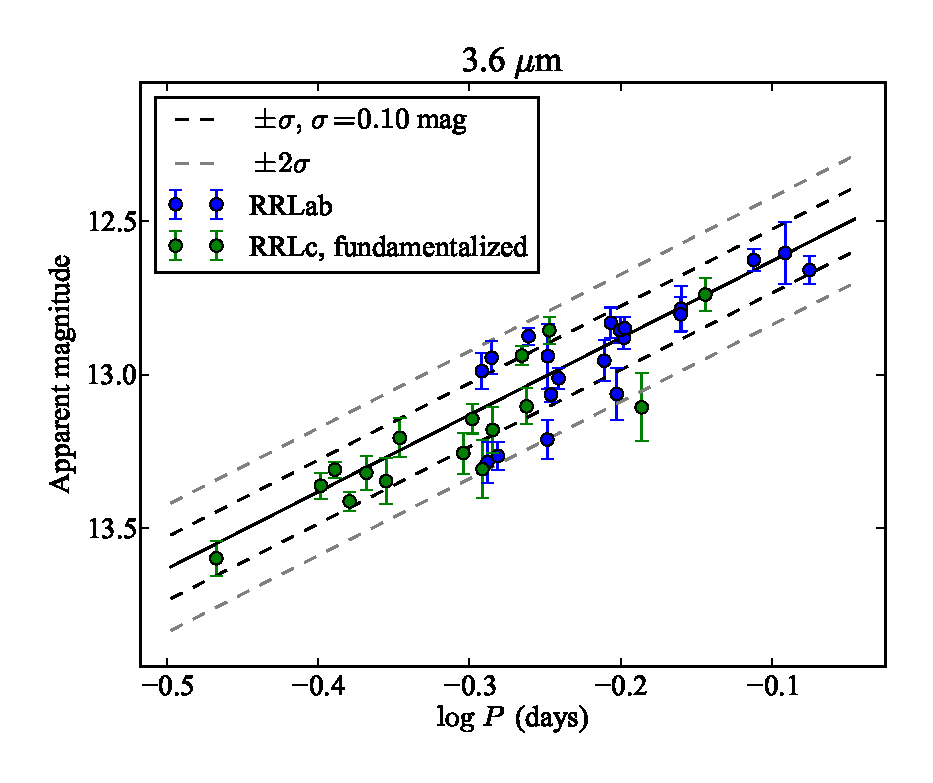
\includegraphics[width=80mm]{PL_3p6.eps} &
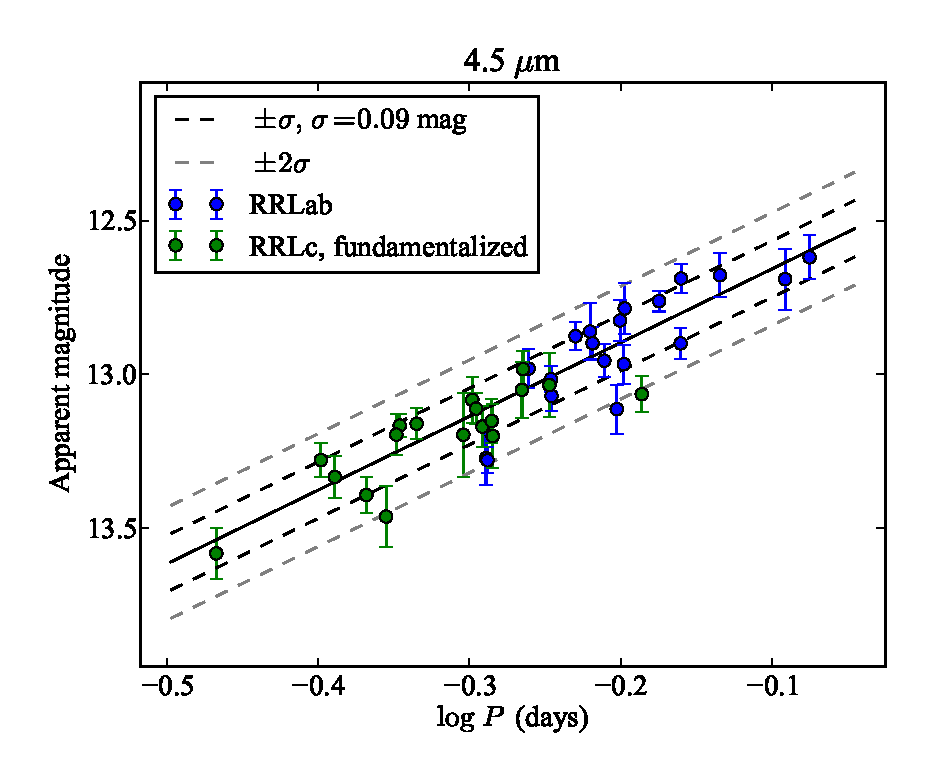
\includegraphics[width=80mm]{PL_4p5.eps} \\
\end{array}$
\caption{The RR Lyrae period-luminosity relation for $\omega$ Cen in [3.6] and [4.5]. The blue data points are RRab's, the green are RRc's with fundamentalized periods, and the flanking lines are 1 and 2$\sigma$.}
\label{fig:pl_relations}
\end{center}
\end{figure}

\begin{figure}
\begin{center}$
\begin{array}{cc}
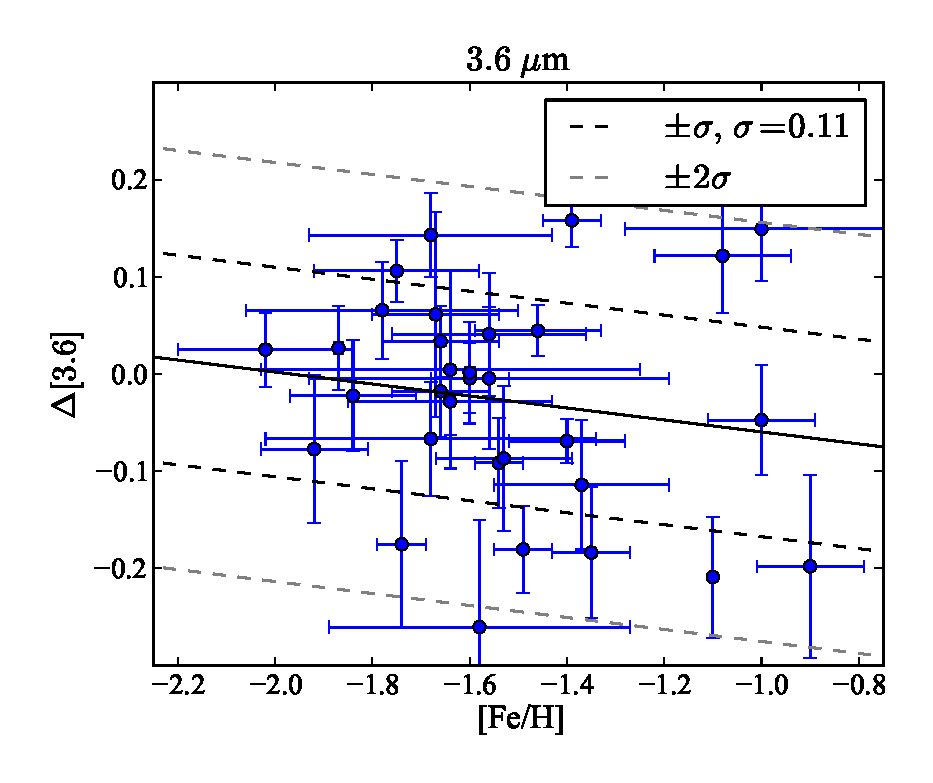
\includegraphics[width=80mm]{Metallicity_3p6_Rey.eps} &
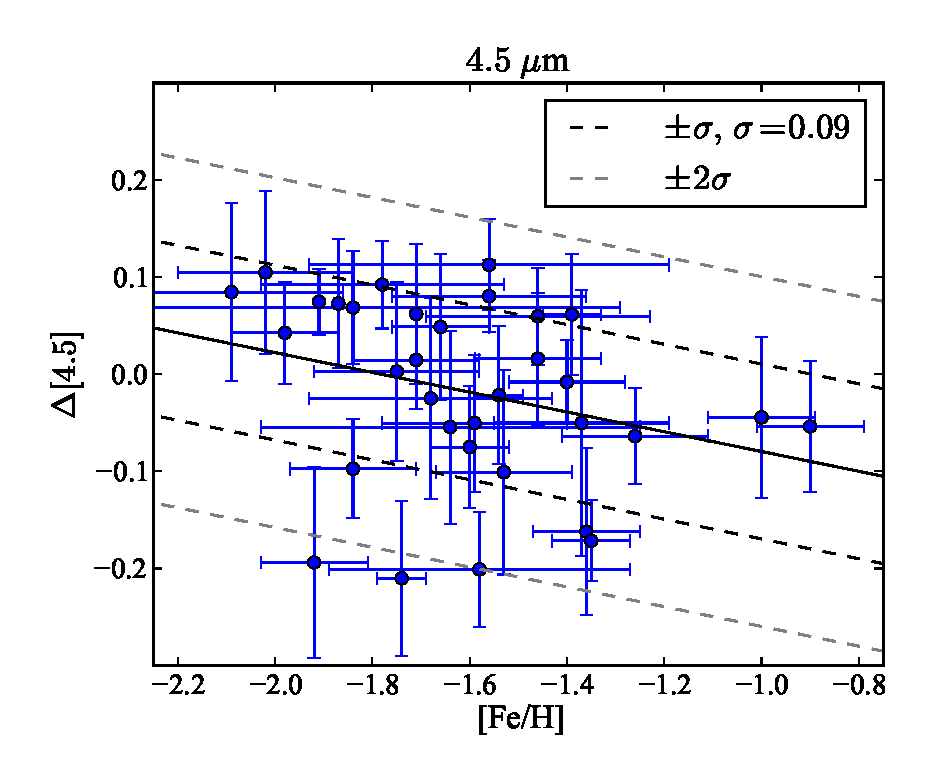
\includegraphics[width=80mm]{Metallicity_4p5_Rey.eps}\\
\end{array}$
\caption{Metallicity vs. PL residuals for $\omega$ Cen in [3.6] and [4.5] using photometric metallicities from Rey et al. (2000). The flanking lines are 1 and 2 standard deviations.}
\label{fig:phot_metal_residuals}
\end{center}
\end{figure}

\begin{figure}
\begin{center}$
\begin{array}{cc}
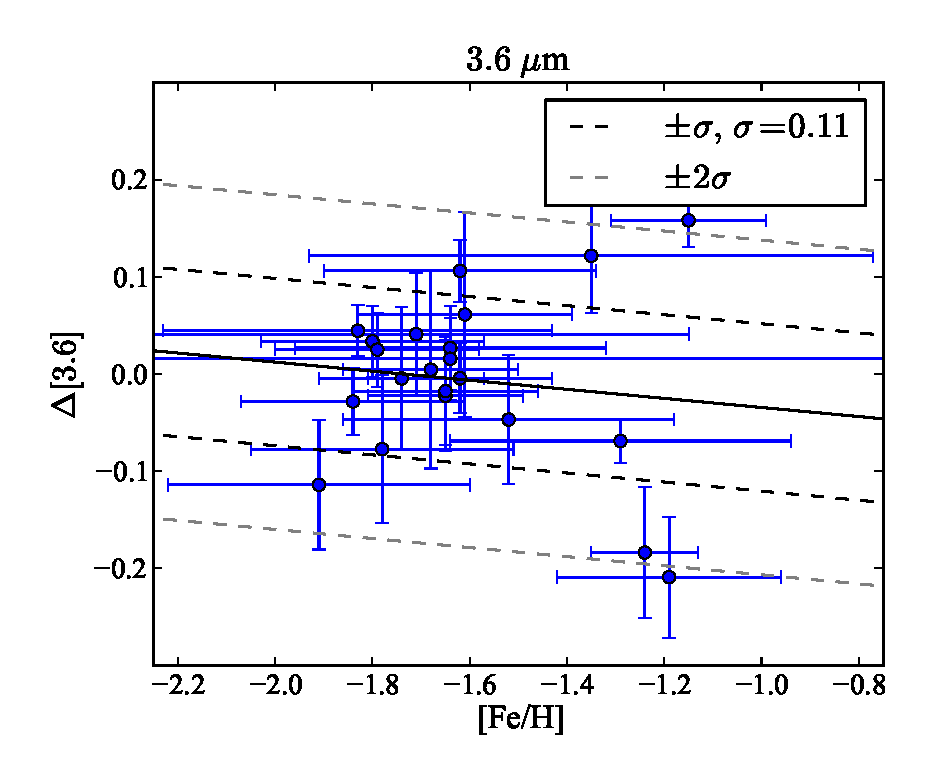
\includegraphics[width=80mm]{Metallicity_3p6_Sollima.eps} &
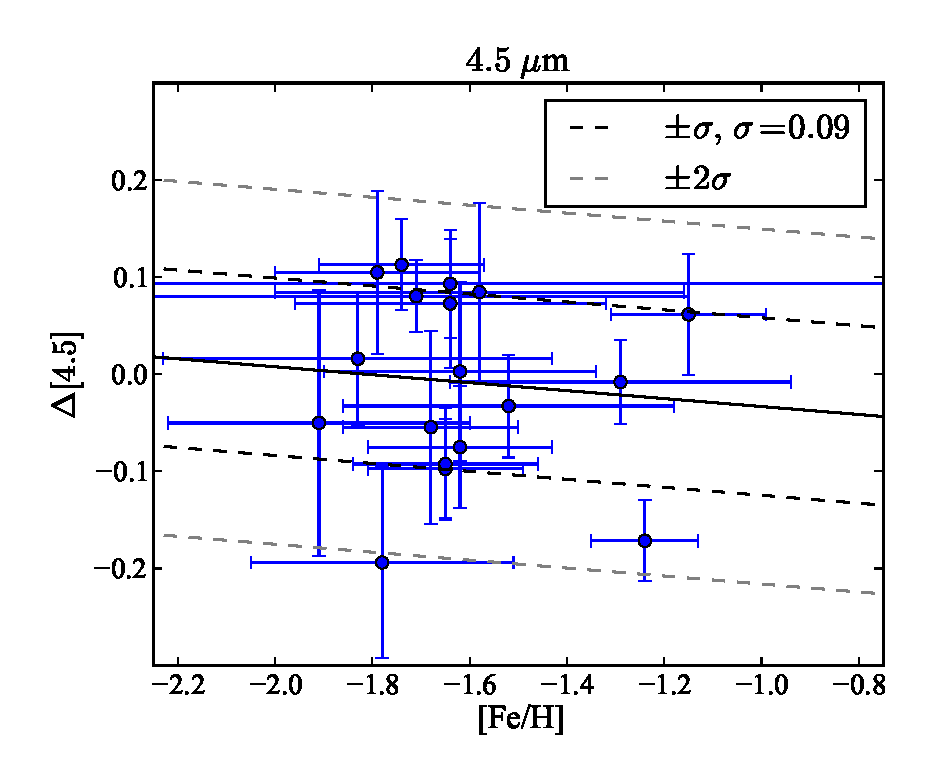
\includegraphics[width=80mm]{Metallicity_4p5_Sollima.eps} \\
\end{array}$
\caption{Metallicity vs. PL residuals for $\omega$ Cen in [3.6] and [4.5] using spectroscopic metallicities from Sollima et al. (2006). The flanking lines are 1 and 2 standard deviations.}
\label{fig:spec_metal_residuals}
\end{center}
\end{figure}

\begin{figure}
\begin{center}$
\begin{array}{cc}
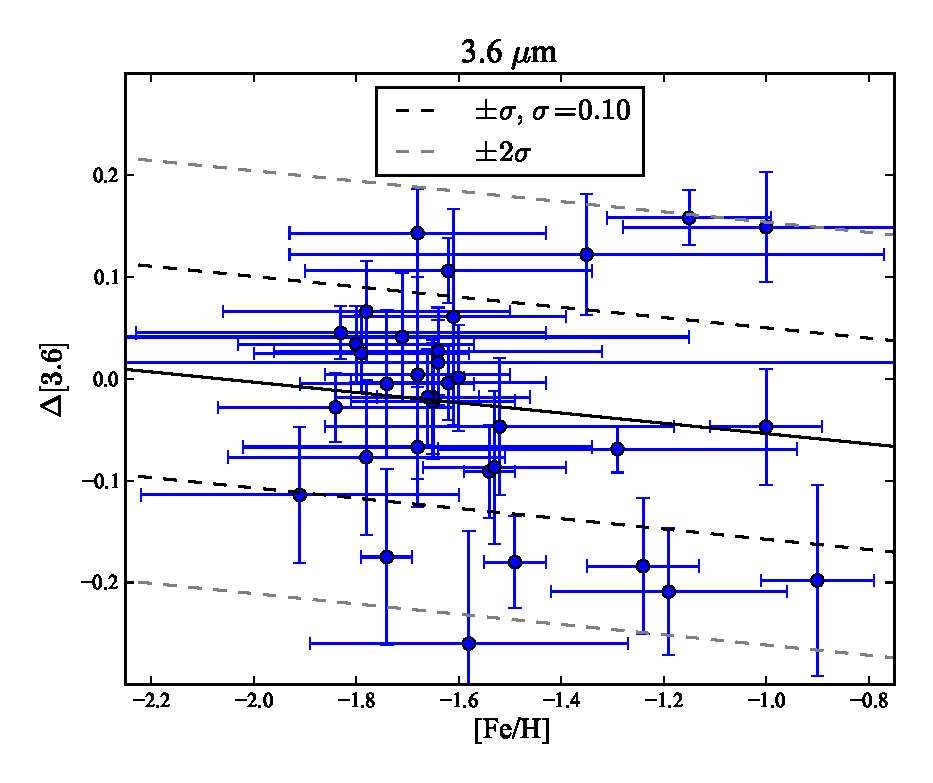
\includegraphics[width=80mm]{Metallicity_3p6.eps}& 
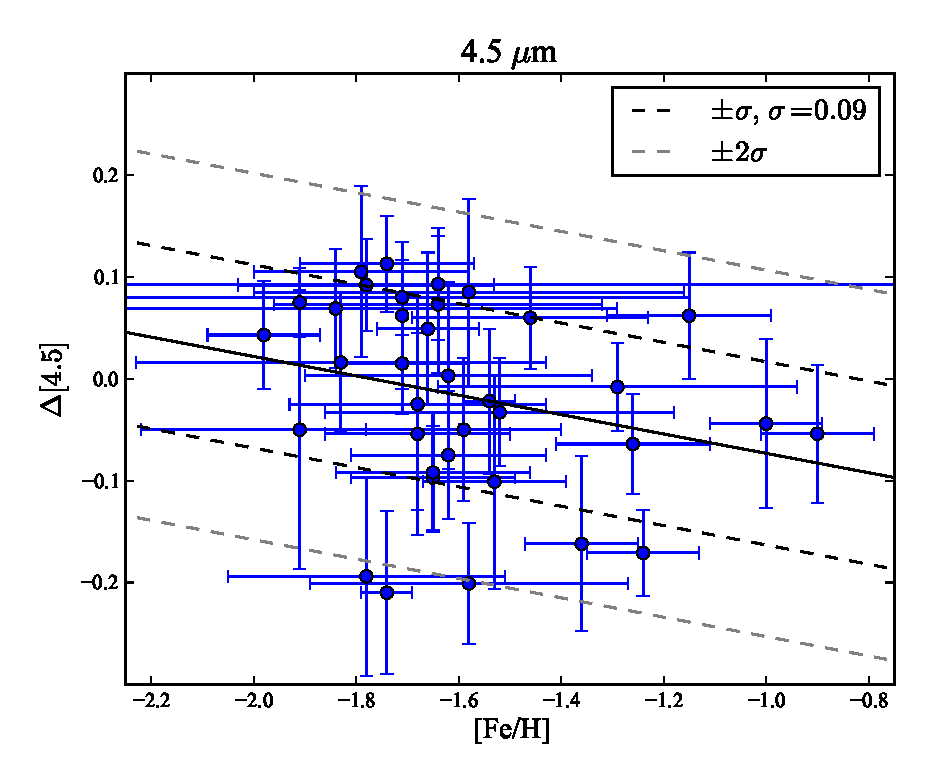
\includegraphics[width=80mm]{Metallicity_4p5.eps}\\
\end{array}$
\caption{Metallicity vs. PL residuals for $\omega$ Cen in [3.6] and [4.5] using combined metallicity catalogs, favoring spectroscopic when both are available. The flanking lines are 1 and 2 standard deviations.}
\label{fig:metal_vs_residuls}
\end{center}
\end{figure}

%%%%%%%%%%%%%%%%%%%%%%%%%%%%%%%%%%%%%%%%%%%%%%%%%%


% Don't change these lines
\bsp	% typesetting comment
\label{lastpage}
\end{document}

% End of mnras_template.tex